% Source :

\documentclass{article}
\usepackage{pgfplots}
\usetikzlibrary{mindmap,trees, backgrounds}

\begin{document}
\section{Introduction}

\begin{figure}[h]
\makebox[\textwidth][c]{
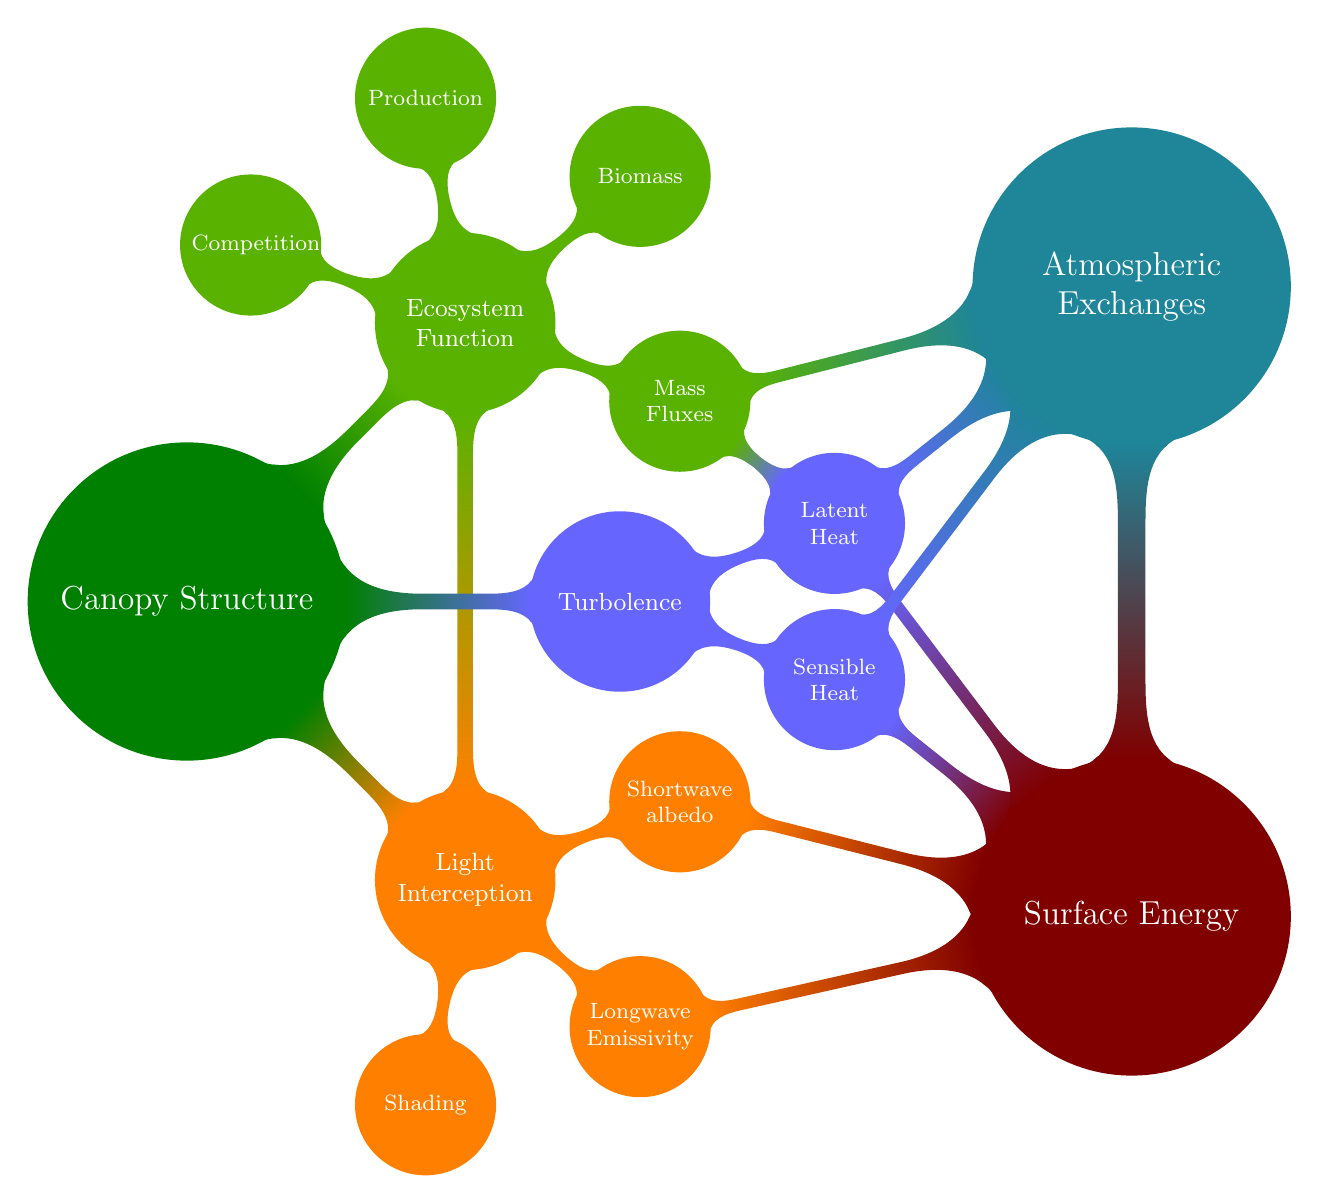
\begin{tikzpicture}
%%%%%%%%%%%%%%% CANOPY STRUCTURE
  \path[mindmap,concept color=green!50!black, text=white]

    node[concept](struct) at (0,0){Canopy Structure}
            child[grow = -45, concept color = orange]{
            node[concept](light){Light Interception}
                    [clockwise from = 20]
                    child{node[concept](alb) {Shortwave albedo}}
                    child{node[concept](lw){Longwave Emissivity}}
                    child{node[concept](shade){Shading}}
                    }
        %----------------------------------------------------------
            child[grow = 45, concept color = green!50!yellow!70!black]{
                node[concept](func){Ecosystem Function}
                    [counterclockwise from = -20]
                    child{node[concept](massflu) {Mass Fluxes}}
                    child{node[concept](biom) {Biomass}}
                    child{node[concept](prod){Production}}
                    child{node[concept](comp) {Competition}
                        child{}}
                    }
        %----------------------------------------------------------
            child[grow = 0, concept color = blue!60!white]{
                node[concept](rough) at (0.5,0){Turbolence}
                    child[grow = 20]{node[concept](lh){Latent Heat}}
                    child[grow = -20]{node[concept](sh){Sensible Heat}}};
        %----------------------------------------------------------

%%%%%%%%%%%% ATMOSPHERE
  \path[mindmap,concept color=blue!80!white!60!green, text=white]
    node[concept](atmos) at (12,4){Atmospheric Exchanges};

%%%%%%%%%%%% ENERGY
  \path[mindmap,concept color=red!50!black, text=white]
    node[concept](energy) at (12,-4){Surface Energy};

%%%%%%%%%%%%% MAKING SECONDARY CONNECTIONS 
  \newcommand{\conngreentoorange}{to[circle connection bar switch color=from (green!50!yellow!70!black) to (orange)]}
  \newcommand{\connredtoorange}{to[circle connection bar switch color=from (red!50!black) to (orange)]}
  \newcommand{\connredtoblu}{to[circle connection bar switch color=from (red!50!black) to (blue!60!white)]}
  \newcommand{\connazuretoblu}{to[circle connection bar switch color=from (blue!80!white!60!green) to (blue!60!white)]}
  \newcommand{\connazuretogreen}{to[circle connection bar switch color=from (blue!80!white!60!green) to (green!50!yellow!70!black)]}
  \newcommand{\connazuretored}{to[circle connection bar switch color=from (blue!80!white!60!green) to (red!50!black)]}
  \newcommand{\connblutogreen}{to[circle connection bar switch color=from (blue!60!white) to (green!50!yellow!70!black)]}
  \begin{pgfonlayer}{background}
    %\draw [circle connection bar ]
      \path (func)  \conngreentoorange (light);
      \path (energy)\connredtoorange (alb);      
      \path (energy)\connredtoorange (lw);
      \path (energy)\connredtoblu (sh);
      \path (energy)\connredtoblu (lh);
      \path (atmos) \connazuretoblu (lh);
      \path (atmos) \connazuretoblu (sh);
      \path (atmos) \connazuretored (energy);
      \path (atmos) \connazuretogreen (massflu);
      \path (lh) \connblutogreen (massflu);
  \end{pgfonlayer}
\end{tikzpicture}}
\end{figure}

\end{document}